\cleardoublepage

\chapter{Estado del Arte de la Domótica}
\label{ch:Capitulo2}

Como definición, el término 'domótica' proviene de la unión de las palabras \verb|domus| ('casa' en latín) y \verb|-tica| (de 'automática', palabra en griego que significa ‘que funciona por sí sola’). De manera más técnica y extensa se puede expresar por domótica, al conjunto de sistemas que hacen de una vivienda un edificio inteligente, aportando servicios de gestión energética, seguridad, bienestar y comunicación, y que pueden estar integrados por medio de redes interiores y exteriores de comunicación, cableadas o inalámbricas, y cuyo control goza de cierta ubicuidad, desde dentro y fuera del hogar. De esta definición no se desglosa nada que concuerde con los problemas descritos en el capítulo~\ref{ch:Capitulo1}. 'Para que una casa funcione por sí sola', no parece estrictamente necesario que, lo que la casa hace, lo tenga que saber y gestionar una persona ajena a la casa, más concretamente, una organización. Si los datos generados, que definen cómo la gente usa el sistema son enviados y procesados fuera del hogar, no existen garantías plenas de que una persona ajena a la unidad familiar pueda visualizar lo que ocurre dentro, desde fuera. No se busca demonizar a las compañías que ofrecen soluciones domóticas, pero sus practicas exponen a las personas a estos riesgos. En cuanto a funcionar de forma autónoma, se podría entender que un sistema es autónomo si, independientemente de factores externos al sistema, éste puede seguir realizando sus funciones fundamentales de manera normal e indefinida en el tiempo. Pero si la solución pasa por un servicio externo y no por las capacidades de la propia casa, eso significa que este sistema no es capaz de operar por su cuenta propia si el proveedor de servicio externo falla.

\vspace{1cm}

Sobre esta dependencia de servicios en la nube surge el paradigma de \verb|edge comupting|, donde los datos registrado por sensores y acciones de actuadores de dispositivos de \gls{iot}, son procesados en niveles más cercanos al lugar donde ocurren en lugar de ser enviados por la red de internet a centros de procesamiento. La estrategia de delegar el procesamiento en los niveles más bajos de un despliegue de \gls{iot}, en lugar de subir toda la información a la red para ser procesada y luego recibir la respuesta, surge como solución a varios problemas fundamentales del procesamiento en la nube. En la figura, extraída del articulo 'Internet of Things (IoT): A vision, architectural elements, and future directions'~\cite{gubbi2013internet}, puede observarse un despliegue de \gls{iot} cuyo procesamiento de datos esta centralizado en la nube.

\vspace{0.5cm}
\begin{figure}[hbt!]
\label{iotCloundComputing}
\centering
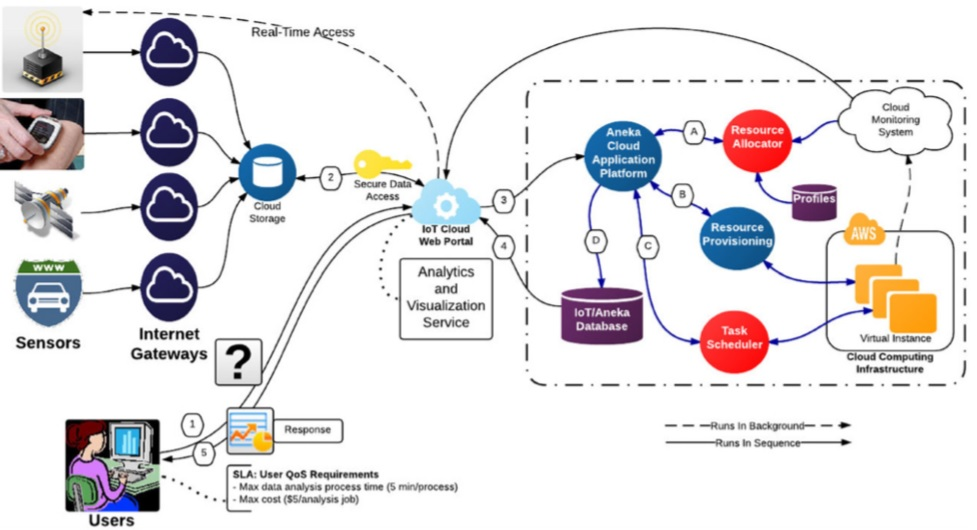
\includegraphics[height=3.5in]{figures/iotCloudComputing.jpg}
\caption[Un modelo de interacción end-to-end entre varios actores en un \gls{framework} de nube centralizado]{Un modelo de interacción end-to-end entre varios actores en un \gls{framework} de nube centralizado}
\end{figure}

Un primer problema de este esquema es la latencia. Si un elemento sensor que actúa como disparador de un elemento actuador debe esperar a que la información del sensor sea enviada a la nube, procesada para evaluar si dicha información implica que se active el actuador, y enviar de nuevo desde la nube dicha señal al actuador, en todo este proceso se genera un espacio de tiempo, que según que circunstancias puede no ser viable, por ejemplo, en un coche autónomo el sistema de frenado cuando va a colisionar con un peatón. A nivel doméstico, otro ejemplo que requiere de un tiempo de respuesta mínimo podría ser una puerta que se cierra mientras que en el proceso una persona pone su mano en el marco y un sensor de presión detecta que debe interrumpir el cerrado. Estos retrasos de respuesta producidos por la latencia son asumibles en la mayoría de los casos de uso de dispositivos de domótica ya que no requieren esta inmediatez de proceso.

\vspace{1cm}

El segundo problema de los esquemas \gls{iot} centrados en la nube, es una cuestión energética. Los centros de procesos de datos, donde se almacenan las plataformas y servicios que gestionan los despliegues de \gls{iot} requieren de infraestructuras de suministro eléctrico ya que ejecutan servicios basados en internet de en una enorme escala. Si el proceso de datos se puede hacer en las fuentes del origen de los datos, conocidos como nodos, o en los concentradores de dichos \verb|nodos|, conocidos como \verb|gateways|, puede reducirse la cantidad de potencia de procesamiento requerida en los servidores finales. Delegar el procesamientos de datos, su almacenamiento temporal o la toma de decisiones en los flujos de ejecución de un proceso en los niveles inferiores de un despliegue de \gls{iot} distribuye el consumo energético a lo largo del despliegue en vez de concentrar todo el proceso (así como la mayor demanda energética) en un único punto. El distribuir la energía no reduce la cantidad total de energía que se usa en un despliegue de \gls{iot}, sin embargo, los elementos inferiores del despliegue como los nodos, pueden en su mayoría estar programados en muchas circunstancias para entrar en modos de hibernación, o directamente apagarse cuando no son necesarios, reduciendo el consumo, y eso incluye a la cantidad de proceso que la nube ha delegado en ellos. La estrategia de \verb|edge computing| ayuda a esta distribución de energía como se explica en el articulo 'The Promise of Edge Computing' sobre las ventajas del procesado de datos en \verb|network edge| en lugar de completamente en la nube~\cite{shi2016promise}.

\vspace{1cm}

Sobre el planteamiento de despliegues de \gls{iot} centralizados en la nube, también se debe considerar los costes de ancho de banda de la información trasmitida a través de la red. Cada protocolo de comunicación dispone de ventajas que les hacen más aptos para cada escenario. En la capa de trasporte definidas en el RFC 1122 de 'Requirements for Internet hosts'~\cite{braden1989requirements} encontramos dos protocolos que abordan la transferencia de información mediante cabeceras de confirmación como es el caso de \gls{tcp} o con un envío sin confirmación como \gls{udp}. Mientras que el primero es muy verboso, y manteniendo una confiabilidad en los mensajes enviados, pudiendo asegurarse la integridad de los contenidos de los datagramas enviados en los paquetes, y reenviando dichos paquetes en caso de perdida durante el envío, esto genera un mayor requisito del ancho de banda necesario. \gls{udp} en cambio es más ligero al desprenderse de estas cabeceras de verificación; por supuesto, esto genera habitualmente que se pierdan paquetes en los envíos, pero no representa un problema si el flujo de información es constante en el tiempo y la pérdida puntual de información no tiene un impacto real en la comunicación. Suponiendo un sensor que toma medidas de manera continua sobre un parámetro concreto, se puede obviar puntualmente fallos en la comunicación si seguidamente tras el fallo se suceden datos correctos. Esta estrategia es aplicada habitualmente en tecnologías de streaming, donde la pérdida de un fotograma es apenas apreciable por el usuario que visualiza el contenido de un vídeo. 

\vspace{1cm}

En escenarios donde una comunicación de un despliegue \gls{iot} requiera de seguridad adicional, los protocolos de transferencia como \gls{http} o \gls{mqtt} requieren del uso del protocolo de transporte \gls{tcp}, ya que las cabeceras adicionales que incluye permiten que la comunicación se establezca con garantías de confiabilidad y técnicas de seguridad como cifrado en los mensajes enviado, verificación de envío y recepción y no repudio. Esto tiene un efecto en la congestión del ancho de banda de las redes de comunicación y su aplicación debe considerar el impacto en los canales de comunicación que supone el uso de un protocolo como \gls{tcp} que es más pesado que el protocolo \gls{udp}. En el documento 'Throughput Analysis and Measurements in IEEE 802.11 WLANs with TCP and UDP Traffic Flows'~\cite{bruno2007throughput}, los resultados de pruebas indican que el rendimiento total del protocolo \gls{tcp} es independiente del número de conexiones abiertas, y su tráfico agregado se modela como dos flujos saturados, mientras que el del protocolo \gls{tcp}, para una cantidad n de flujos, obtienen casi n veces el rendimiento agregado logrado en los flujos \gls{tcp}. Considerando esta conclusión, el protocolo \gls{udp} es más apto para un despliegue multitudinario de dispositivos que el protocolo \gls{tcp}. Si bien es cierto que, en domótica, es difícil que exista un número extenso de dispositivos conectados simultáneamente en la red del hogar.

\vspace{1cm}

Y uno de los problemas cuyo impacto posee tanto una vertiente legal que tecnológica es la privacidad de los datos enviados a la nube. En este punto en particular, los despliegues de \gls{iot} basados en procesamiento en la nube, son los que poseen más riesgos, ya que al viajar los datos a través de la red de internet, están más expuestos a la interceptación por terceros. En domótica, los datos transferidos por la red están relacionados con los objetos cotidianos equipados con sensores y actuadores que permiten adquirir información sobre los usuarios de manera automática, permitiendo la recopilación de datos que conduce a inferencias sobre la persona monitorizada. Esto permite crear perfiles de consumidor mediante la denominada técnica de "fusión de sensores". Los datos obtenidos en despliegues de domótica pueden parecer datos no personales, pero permiten definir el comportamiento de una persona y crear identidades virtuales que son usadas en estrategias de marketing por las empresas de consumo~\cite{iotDataProtection}. En el capítulo \ref{ch:Capitulo1.1}, se mencionan tres marcas que ofrecen suites de domótica a nivel internacional. Se trata de actores con gran presencia en el sector de la domótica de consumo para el hogar. Su importancia es tal, que están definiendo con sus productos el futuro de la domótica, y todas ellas, en mayor o menor media, se ven envueltas en escándalos sobre el tratamiento de datos de usuarios. En el siguiente apartado, profundizaremos en cómo estas empresas abarcan la normativa impuesta en Europa y los estados miembros que recientemente ha obligado a muchas empresas a adoptar su marco de actuación para adecuarse a la norma del \gls{rgpd}.

\section{Políticas de privacidad de marcas con gran presencia de mercado}
\label{ch:Capitulo2.1}

Todo lo que gira en torno al concepto 'política de privacidad' o 'términos de condiciones de uso', se puede traducir, como la experiencia nos ha enseñado, a una aceptación a ciegas de los contratos por parte del usuario final. Esta causa viene motivada principalmente por la complejidad de obtener, abstraer y entender los extensos puntos que conforman estos textos legales, que siguen estando muy lejos de ser amigables. Observamos como se presentan dichos textos en las siguientes marcas, para entender las dificultades que un usuario debe enfrentar si quiere saber exactamente qué está contratando.

\vspace{1cm}

\verb|Amazon Alexa (Amazon Movile LLC)|: Su política de privacidad~\cite{alexaprivacy} indica que se suben grabaciones del usuario a sus servidores para ser procesadas en sus sistemas de reconocimiento de voz y compresión de lenguaje. No se indica expresamente que dichas grabaciones, además, son incluidas en procesos de entrenamiento de \gls{machinelearning} para mejorar su aplicación. Se indica además, que su dispositivo no graba continuamente, salvo por reconocimiento del comando de activación (generalmente el nombre del dispositivo), pero tampoco se especifica cuánto tiempo graba, ni qué hace con las filtraciones de voz de otras personas que estén presentes. La cláusula de servicios a terceros resulta bastante ambigua, pero indica que cualquier cesión de permisos a una aplicación de terceros que se integre con Amazon, podrá requerir datos a la misma. Se pueden encontrar más detalles en sus condiciones de uso~\cite{Alexauserconditions}. En la misma podemos observar adicionales cláusulas anidadas que redirigen a nuevos enlaces como las condiciones de uso de Amazon España~\cite{Alexaspainuserconditions}. Al final es realmente difícil saber a qué se atiene un usuario que adquiere este producto. Su aplicación de móvil también requiere un abanico realmente extenso de permisos en el \gls{so} de un Smartphone/tablet, incluyendo gestión de cuentas en el dispositivo (añadir o eliminar cuentas), accesos a contactos, ubicación, mensajería, llamadas, almacenamientos, dispositivos de entrada/salida y un largo etcétera que puede consultarse en la tienda de aplicaciones correspondiente de Android/iOS.

\vspace{1cm}

\verb|GoogleHome (Google LLc.)|: Google lleva años intentando mejorar sus servicios respecto a las leyes europeas de protección de datos. Aun habiendo sonados casos de tratamiento ilegal de \gls{dcp} que han terminado en sanciones a la compañía, como las de la \gls{aepd} que alcanzan hasta 900.000 euros tal y como recogía en esta noticia del medio ~\cite{j.m.sanchez_2014}, aun así, eso no ha frenado la expansión de la compañía a lo largo del mundo. Todo ello seguramente condicionado a su presencia internacional, ya que en algunos países son además proveedores de servicios e infraestructuras de instituciones públicas como ocurre en la \verb|Universidad Complutense de Madrid|, así como proyectos conjuntos como la digitalización de la Biblioteca Complutense~\cite{bibliotecaucmgoogle8}. En el campo de la domótica, lo que respecta a su política de privacidad en su aplicación \verb|Google Home|, se remite al usuario a las condiciones generales~\cite{googleprivacy} de la compañía de \verb|Google LLc|, para información más concreta sobre el producto, es necesario buscar información en la página de ayuda de Google~\cite{googlenestsecurityandprivacy}. En la misma, se afirma la intención de recoger datos (no se especifican de qué naturaleza), con el fin de usarse en \gls{machinelearning}. Se confirma que podrían existir aplicaciones de terceros que nutran a \verb|Google| con más datos (tampoco se especifican qué datos ni qué aplicaciones de terceros). Aun así, ofertan la posibilidad de gestionar los datos almacenados en su gestor de actividad y en caso de tener la configuración por defecto de recogida de datos que \verb|Google| utiliza en los \gls{so} de Android, los resultados son, como poco, inquietantes. Un sistema de domótica de esta compañía es perfectamente capaz de determinar con exactitud casi toda la vida diaria de una casa, incluyendo cuándo se duerme, cuándo se come, quien esta en el hogar, y qué actividades se han desarrollado.

\vspace{1cm}

\verb|Xiaomi Mi (Xiaomi INc.)|: La empresa china que ha irrumpido en el mercado europeo gracias a sus aplicaciones con interfaz amigable, presentaciones de productos semejantes a las ejecutadas por compañías como \verb|Apple| y precios competitivos, que además admiten múltiples dispositivos clónicos de fabricantes no adscritos a la marca de \verb|Xiaomi| también está haciendo sus adaptaciones para operar en Europa bajo el marco de la \gls{rgpd}: su política de privacidad~\cite{xiaomyprivacy} sobre la recopilación de datos es, cuanto menos, ambigua, usando frases como, "podemos recopilar la totalidad o una de la parte que usted nos proporciona", y en lo que respecta a de qué manera se utiliza dicha información, es tan extensa que sólo remarcaremos que aparece el nombre de la compañía \verb|Facebook| en uno de los puntos. Se afirman en que no se venderán los \gls{dcp} a terceros salvo aceptación del usuario. La estrategia de la compañía de \verb|Xiaomi| en su aplicación pasa por ofertar toda clase de servicios, incluyendo chats, foros, pagos en la plataforma de AliPay, etc. La consecuencia de estos servicios genera la tabla más larga de permisos necesarios en un smarthpone/tablet de los ejemplos mencionados. Definitivamente, aquel usuario que instale esta aplicación y permita todas esta condiciones puede olvidarse de su privacidad.


\vspace{1cm}

El uso extensivo en todas las marcas de un término tan general como \gls{machinelearning} es ambiguo, ya que en ninguno de los casos se especifica qué tipo de modelos analíticos se pretenden crear, aunque se menciona que el objetivo es mejorar sus servicios. Bajo este argumento, un usuario puede entender que ha pagado por un producto una cantidad concreta de dinero, pero el uso de ese producto, generara unos beneficios para la empresa que se verán de nuevo retribuidos en el usuario con un mejor servicio. Pero existen mejoras que serán exclusivas para la empresa y no repercutirán en el usuario de forma directa, puede que de ninguna forma incluso, como ocurre con modelos analíticos de datos orientados a marketing, que facilitarán a la empresa la capacidad de expandir su negocio y beneficiarse. No es que este intercambio de beneficios sea incorrecto, pero se inclina a favorecer a la empresa sobre el usuario en la mayoría de los casos. En general toda plataforma domótica tratara de nutrir \gls{dataset} con técnicas de \gls{machinelearning} para mejorar la calidad de servicio; aun así, existen plataformas basadas en licencias de código abierto o licencia libre que permiten al desarrollador determinar si dicho flujo de datos puede usarse para este fin o deben permanecer en manos de los usuarios finales. En el siguiente apartado~\ref{ch:Capitulo2.2} se enumeran algunos \gls{framework} comunes en proyectos de \gls{iot} y cómo concuerdan con esta preocupación sobre los \gls{dcp}.


\section{Frameworks disponibles para la gestión de IoT para SmartHomes}
\label{ch:Capitulo2.2}

Un planteamiento recurrente en el diseño de una solución basada en software es acelerar el proceso de desarrollo e implementación utilizando un \gls{framework}. Es una buena idea. Estas herramientas están, en su mayoría, profundamente documentadas para exprimir sus capacidades al máximo, disponen de versionados y revisiones (en mayor o menor medida) que fortalecen tanto su seguridad, robustez, e implementación. Poseen una buena abstracción del hardware en el que se ejecutan, sus servicios son modulares y su arquitectura es escalable. En ocasiones están basados en software libre y/o gratuito, y disponen de una comunidad activa de usuarios a los que poder exponer dudas. Éstas son cualidades muy importantes, mas allá de las capacidades técnicas que cada opción pueda ofrecer.

\vspace{1cm}

En despliegues de \gls{iot} es importante determinar el alcance en conectividad que se desea alcanzar y volumen de datos a tratar. Existen \gls{framework} pensados para interconectar ingentes cantidades de dispositivos en grandes extensiones de terreno y bajo el peso de un abrumador volumen de datos que procesar como es el caso de las SmartCities, o la infraestructura del sector primario y secundario. En algunos casos, el alcance es tan extremo que el concepto de \gls{iot} evoluciona a \gls{ioe} y se requiere la presencia de grandes actores tecnológicos, y sus soluciones, para abarcar estos proyectos, como es el caso del framework \verb|IBM BlueMix| de IBM, el \verb|Cisco Virtualized Packet Core| de Cisco, \verb|AWS IoT| de Amazon o \verb|Azure IoT| de Miscrosoft, por mencionar algunos ejemplos de este calibre. Estos \gls{framework} no fueron diseñados pensando en reducidos entornos como los de un hogar, y aunque son compatibles, el tiempo necesario en formación para su uso queda fuera de las capacidades y expectativas de un proyecto de las características que aquí se recoge. Sin embargo, también se dispone de un amplio abanico de opciones a un alcance más acorde a lo esperado de una solución domótica.

\vspace{1cm}

Ha de establecerse una serie de criterios que han de aplicarse al valorar las opciones de \gls{framework} disponibles, los cuales deben estar en consonancia con la motivación de este proyecto. Antes de realizar cualquier evaluación sobre las bondades de cada plataforma, se debe recordar que en la solución a buscar, se intenta evitar el uso de servicios en la nube o dependencias de \gls{api}s externas. Esto responde al objetivo de aislar la suite domótica a desarrollar, de la red de internet, evitando esa dependencia para su operatividad. Por supuesto, no es el objetivo crear una plataforma desconectada, ya que se espera poder operar de forma remota los dispositivos desde fuera del ámbito de la red local del hogar. Además, debe disponer de un licenciamiento de código libre y gratuito; en otro caso, estaríamos contraviniendo la naturaleza de este proyecto. Y no menos importante, están los costes económicos que deben asumirse al crear el prototipo.

\vspace{1cm}

\verb|FIWARE|: Esta catalogada como una plataforma de código abierto que agrupan un set de estándares universales para el contexto de gestión de datos~\cite{whatisfiware}. Se sustenta en la ejecución de un \gls{framework} ejecutado sobre un \gls{docker}, que puede ser alojado localmente en un ordenador dentro del hogar, y aunque esta solución está orientada a procesar datos en un contexto más extenso que una casa, puede aislarse de la red de internet. Limitan la portabilidad de las aplicaciones a aquellas que se catalogadas 'Powered by FIWARE', y aunque ofrecen una interfaz estándar para los componentes que integren la solución, con el objetivo de eliminar el bloqueo del proveedor de componentes, posee un licenciamiento de código abierto y un entorno  de ejecución no comercial llamado \verb|FIWARE Lab| que permite experimentar sus tecnologías. Estos laboratorios de pruebas están instalados en \gls{docker}s propiedad de la propia compañía de \verb|Fiware| y es ejecutado sobre una instancia de \verb|Open Stack|. Para desarrollar cualquier tipo de despliegue \gls{iot} basado en esta tecnología, es obligatorio integrar en el desarrollo de la aplicación el llamado 'Orion Context Broker Generic Enabler', el cual habilita la gestión de información contextual izada de manera descentralizada y de a gran escala.

\vspace{0.5cm}
\begin{figure}[hbt!]
\label{fiwarecontext}
\centering
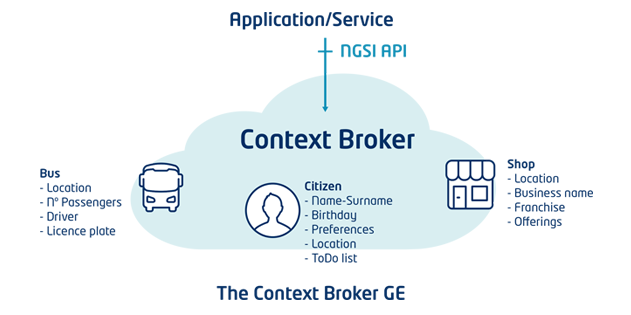
\includegraphics[height=3.5in]{figures/fiware_context_broker.png}
\caption[Broker de contexto de información de Fiware]{Broker de contexto de información de Fiware}
\end{figure}

Facilita el \gls{api} restful \verb|FIWARE NGSIv2| que permite ejecutar queries, actualizaciones o suscripciones a cambios de contexto de la información. Este contexto de la información permite realizar consultas sobre sensores en distintos escenarios en función de un mismo criterio, tal y como se muestra en la figura, en la cual la misma consulta puede ser ejecutada en varios escenarios definiendo el contexto adecuado. Esta estrategia no permite explotar su potencial en un proyecto centrado en la domótica de un hogar, que no esta planteado para beneficiarse de contextos de datos recogidos por sensores ajenos al propio hogar.

\vspace{0.5cm}
\begin{figure}[hbt!]
\label{fiwarechangecontext}
\centering
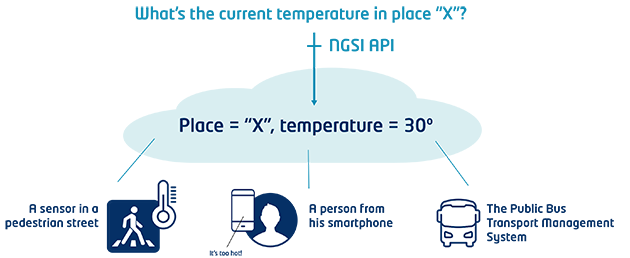
\includegraphics[height=2.6in]{figures/fiware_context_change.png}
\caption[Acceso a la información en múltiple contextos con Fiware]{Acceso a la información en múltiple contextos con Fiware}
\end{figure}


\vspace{1cm}

\verb|OpenHab|: Recomendado frecuentemente en foros y ponencias de \gls{iot}, bajo el nombre de \verb|Open Home Automation Bus|. Esta plataforma dispone de manuales de instalación para convertir un ordenador en un centro de control de domótica, incluyendo la propia Raspberry Pi con una imagen ya configurada~\cite{openHabRaspberryPi}. La documentación detalla la definición de un modelo de desarrollo orientado a objetos, flexible y escalable, donde las llamadas \verb|things|, representan a los dispositivos físicos, que incluyen las propiedades para gestionar sus canales de comunicación así como \verb|items| que representan la capacidades y propiedades de los automatismos del hogar. También se proponen reglas, que definen comportamientos en función de los disparadores asignados por el usuario. De esta forma, puede automatizarse el apagado de las luces de una estancia si en ésta no hay individuos. Dispone de un extenso abanico de interfaces, incluyendo un chatbot llamado HABot para controlar la suite domótica con un lenguaje natural escrito (Esta misma función ha sido objeto de proyecto en un reciente trabajo de fin de máster de la facultad de informática~\cite{brun2018smart}). Posee una \gls{api} restful que permite una interoperatividad con servicios externos o desarrollos propios y soporte para todas las principales plataformas móviles (Android, IOs, Windows) ya que está programado en Java. No se limita tampoco en interoperatividad con buena parte de servicios y stacks de desarrollo existentes, y dispone de una extensa gama de dispositivos compatibles mediante Add-ons, como, por ejemplo, Chromecast o Philips Hue, otras soluciones domóticas como ‘Max! Home Solution’, o protocolos como \gls{mqtt} o estándares de redes con \gls{tcp}, \gls{udp} o WOL (Wake on LAN) entre otros. De hecho, salvando que su licenciamiento se limita a ser open source, es de lejos, una de las mejores opciones disponibles que cumplen con lo necesario para crear una solución domótica aislada ya que, al no generar dependencias de servicios externos, puede ser operada localmente o de forma remota y dispone de capacidad suficiente en cuanto a soluciones modulares para cubrir los futuros casos de uso que se plantearán. \verb|Open Hab| está en sintonía de los objetivos de este documento, cubre las necesidades de nuestro alcance y mucho más. De hecho, cubre tantas posibilidades y entregan tantos servicios listos para ejecutar, que en las primeras pruebas nos sentimos totalmente vacíos. Perdimos la capacidad de experimentar los distintos niveles que conforman una suite domótica, por que este \gls{framework} ya lo proporcionaba prácticamente todo. Además, su documentación es bastante extensa, quedándose el análisis de otras opciones fuera del tiempo establecido de investigación del estado del arte. Finalmente se decidió no implementarlo.

\vspace{1cm}

\verb|MainFlux|: Se define como una plataforma tecnológica de código abierto y patente libre con licencia Apache 2.0. Incluso ofrece un dispositivo \gls{gateway} para soluciones industriales y de computación desarrollada por la misma \verb|Linux Foundatión|. Esta planteado como \gls{paas} para integrar aplicaciones que interactúan con los nodos mediante un \gls{gateway}. La plataforma, dispone de una versión gratuita para ser alojado localmente en un Docker o un equipo con SO Linux. Su documentación clarifica que el desarrollo de aplicaciones que conectaran a Mainflux se realizaran a través de protocolos bridging (como HTTP, MQTT,WebSocket o CoAP)~\cite{mainfluxdoc}.


La opción de trabajar sin \gls{framework}, aunque supone un mayor esfuerzo, puede despejar ideas preconcebidas que se plantean en las diversas soluciones, dando la opción de experimentar más abiertamente, sin las restricciones tecnológicas impuestas por las aproximaciones de dichos \gls{framework}. En este punto de la documentación los autores decidieron unificar su propio conjunto de servicios y protocolos y desarrollo para crear una solución nueva, enfrentando así los retos que deben resolverse en su totalidad para alcanzar un despliegue de \gls{iot} enfocado a domómotica con la estrategia de \gls{gateway} y nodos.

\section{Estándares y protocolos de comunicación y Stack de servicios}
\label{ch:Capitulo2.3}

Orientando la selección de los servicios, estándares y protocolos necesarios para la creación de un prototipo, que permita alcanzar los objetivos planteados para este proyecto, surge la necesidad de plantear la estrategia de comunicación de dispositivos. Esto implica seleccionar un formato de depliegue de dispositivos en la red que comunica los nodos con el \gls{gateway}. 

\vspace{1cm}

\subsection{Stack de servicios}
\label{ch:Capitulo2.3.1}

Para nuestra estrategia de selección de servicios, se empieza determinando que BBDD que cimentará el resto del stack. Toda aplicación informática se sustenta en primera instancia sobre el almacenamiento de datos de manera persistente. Se segmentan en 2 categorías principales según como se relacionen entre sí dichos datos, esto es: BBDD relacionales, o no relacionales. Además de esta segmentación principal, existen otras características importantes en cuanto a la escalabilidad y diseño de cada modelo. Si consideramos cómo entendemos humanamente los datos necesarios para una suite domótica, una de las primeras impresiones, es que no sabemos con certeza cuántos dispositivos de sensorización o actuadores serán necesarios para cada caso de uso. De hecho, es muy probable que un mismo caso de uso disponga de diferentes combinaciones de dispositivos para alcanzar una solución. Es, sin embargo, bastante obvio que básicamente almacenaremos pocos conceptos atómicos, los principales son: Ubicaciones, dispositivos en las ubicaciones y medidas y/o acciones de los dispositivos.

\vspace{1cm}

En la mayoría de proyectos de \gls{iot} observados en nuestras indagaciones, aparece en escena MongoDB. Es una elección popular gracias a su escalabilidad y flexibilidad, esto permite sortear más fácilmente la problemática de adaptarse y anticiparse a los cambios tan continuos que sufre el escenario del gsl{iot}, ya que aparecen nuevos sensores continuamente, que generan nuevas muestras de datos, con funcionalidades distintas, etc. En una BBDD relacional es difícil realizar iteraciones del modelo de datos de esta manera. Por otro lado, el proceso de analizar unos datos que evolucionan continuamente, no sólo en contenido, sino en forma, hacen que su extracción y procesado se vuelva muy compleja. Las BBDD no relacionales son mas amigables a la hora de definir criterios para extraer informaciones concisas dentro de un documento heterogéneo. Además, MongoDB está pensado para trabajar estrechamente con datos presentados en formato \gls{json}. Esto hace su uso muy conveniente en un entorno de aplicación que se base en estas estructuras de datos como ocurre con los motores de JavaScript (de los navegadores o de servidores) o la mayoría de aplicaciones móviles.

\vspace{1cm}

Destacar este último aspecto es determinante a la hora de seleccionar el entorno de ejecución que usará el servidor de la aplicación de domótica. En este aspecto, existen múltiples estrategias, todas ellas en una primera aproximación válidas. Se puede disponer de un servidor web como Apache o Nginx, programados en lenguaje PHP. Este tipo de servidor es capaz de establecer conexiones por el protocolo HTTP/HTTPS con un cliente solicitante, procesar una determinada información y entregar una respuesta codificada en texto plano para que el software del cliente lo reciba. También puede ser extendido para procesar comunicación mediante \gls{mqtt}, la cual es una excelente alternativa a HTTP/HTTPS dependiendo del contexto, y que analizaremos posteriormente.

\vspace{1cm}

Otra alternativa podría ser NodeJS. El creador de NodeJS tuvo la idea de coger el motor V8 de JavaScript del navegador Google Chrome y montarlo como el núcleo de NodeJS. NodeJS se programa en JavaScript, y representa un cambio de paradigma en la ejecución, puesto que sólo utiliza un hilo de ejecución y procesamiento de entrada y salida asíncronos; lo que evita bloqueos en el procesamiento y ayuda a optimizar los recursos del servidor.  Además, es Open Source, multiplataforma y muy modular, lo cual atrajo y sigue atrayendo a una enorme cantidad de desarrolladores que contribuyen a su crecimiento añadiendo librerías en NPM (Node Package Manager), de forma que hoy en día, NodeJS posee infinidad de utilidades ampliamente testadas a su alcance, fácilmente reutilizables en cualquier proyecto.

\vspace{1cm}

Para el fin que ocupa al proyecto, es útil añadir el \gls{framework} de ExpressJS, ligero y flexible orientado a la creación y exposición de una API REST con el objetivo de atender las peticiones de aplicaciones web y móviles. Esta adición sería casi imprescindible, pues la API básica de utilidades HTTP de NodeJS es muy poco amigable. Sin embargo, juntos, levantar un servidor web y una API REST completa y segura es una tarea asequible con poco más de un centenar de lineas de código. Otras librerías muy útiles y que nos conciernen podrían ser las que permiten integración con servicios como los arriba mencionados MQTT y MongoDB (para la cual está excepcionalmente bien orientado, dada la flexibilidad de JS y su natural compatibilidad con las estructuras de datos JSON).

\vspace{1cm}

\subsection{Protocolos de comunicación}
\label{ch:Capitulo2.3.2}


Mosquitto es un mediador de mensajes que incluye el protocolo MQTT. Además es de código abierto su documentación es extensa y detalla lo que supone una ventaja para los desarrolladores.

\vspace{1cm}

Para discutir sobre las alternativas de comunicación del servidor con los dispositivos, hablaremos del arriba mencionado MQTT. Frente a la simple pero efectiva estrategia de HTTP/HTTPS, en proyectos de gls{iot}, hay un protocolo originalmente ideado por la compañía de IBM de licencia libre enfocado a una conectividad maquina a maquina (M2M), el código de dicho protocolo fue donado en 2011 al proyecto de Eclipse. Mientras que el protocolo HTTP/HTTPS puede manejar volúmenes grandes de información en su transferencia por la red de comunicaciones, el protocolo MQTT requiere menos ancho de banda, está orientado a proyectos con un bajo consumo y que dispongan de poco recursos de procesamiento; lo cual encaja con el enfoque necesario de una suite domótica, donde por ejemplo, si hay que obtener la temperatura de una habitación, todo se reduce a un único dato, un número (posiblemente decimal), o al menos, eso es lo que un usuario espera recibir. Esto implica que, un sensor de temperatura, en algún lugar de la casa, recibe una petición en la red en la que se encuentra de otro dispositivo, toma la medida y la envía a dicho dispositivo.

\vspace{1cm}

Si usamos el planteamiento de un servicio web, el sensor dispondrá de la capacidad de recibir una solicitud en un puerto abierto, cuando reciba la petición adecuada, responderá incluyendo en el cuerpo de la respuesta dicha medida y será procesada en el dispositivo que creó la petición. Esto significa que cada sensor/actuador será por sí mismo un servidor web con un puerto abierto que atiende peticiones de clientes. Si todos los dispositivos están conectados en la misma red, salvo que se apliquen restricciones específicas en el firewall, serán visibles entre sí, pudiendo encadenar llamadas y respuestas entre ellos, o a través de un dispositivo central que se encargue de hacer las solicitudes y cuyas respuestas recibidas sean procesadas para mostrarse en la aplicación móvil.


Desde el planteamiento del protocolo \gls{mqtt}, la estrategia gira en torno al concepto de suscripción de $topics$ o temas, donde los dispositivos publican información de distintos temas y los suscriptores a dichos temas reciben la información cuando es publicada. A nivel físico, todos los clientes se conectan a un punto central, lo que define una topología de estrella (con sus ventajas e inconvenientes). Dicho nodo central es el servidor definido como $broker$, y es el único que sabe a qué topic está suscrito cada cliente. Esto significa que cada uno de los sensores/actuadores de la red ignora al resto de los dispositivos, ya que sólo atienden la comunicación con el broker a través de una conexión gls{tcp} permanente. Esta estrategia es diferente a la usada en el protocolo \gls{http}, ya que no es necesario hacer una petición para recibir información de un cliente. Simplemente el broker da o solicita información en los topics a los que los dispositivos están suscritos. Para proyectos de este tipo, el hecho de que los dispositivos no se relacionen entre sí, dan lugar a una gran ventaja, la escalabilidad. en el año 2014 se ha convertido en un estándar OASIS. \gls{mqtt} soporta cifrado mediante SSL. Es un protocolo fiable. Eso se debe a que tiene implementado \gls{qos}.

\vspace{1cm}

La escalabilidad de una suite domótica es un factor determinante al considerar su implementación. Que los dispositivos que conforman la red puedan cambiar con facilidad su organización, número o capacidades es un valor añadido.


\subsection{Estándares en IoT}
\label{ch:Capitulo2.3.3}

La domótica se remonta a los años 70, uno de los primeros hitos fue el protocolo de comunicaciones X-10~\cite{x10protocolwikipedia} de automatización de dispositivos en la línea eléctrica de un hogar. Con él, se puede utilizar la propia red como canal de comunicaciones mediante ráfagas de pulsos. El ancho de banda de 256 dispositivos simultáneos es una cantidad más que suficiente para interactuar con los dispositivos de un hogar, si calculamos que cada elemento susceptible de ser automatizado como por ejemplo persianas, estufas, enchufes, e interruptores ocupase un espacio de este ancho de banda, seguirían sobrando espacios en un piso de 150 metros cuadrados.

\vspace{1cm}

En pleno 2019 pueden adquirirse los dispositivos necesarios para instalar una red X-10 que incluye interruptores, actuadores, sensores, transmisores, interfaces y unidades de control (todos ellos necesarios para obtener el control completo de la red) por precios con rangos entre 20 a 70 euros por cada elemento. Esto supone inversión elevada si se tiene en cuenta un hogar de varias habitaciones. Hay que considerar además ciertas limitaciones como que cada controlador es capaz de manejar un número limitado de dispositivos.En cuanto a las aplicaciones necesarias para gestionar el sistema, X-10 posee alternativas de código libre para su desarrollo como \verb|Minerva|. También existen interfaces hardware que traducen el protocolo X-10 a \gls{api}s de servicios web como el dispositivo \verb|ioBridge| que supuso una disrupción en el ámbito del \gls{iot} y la automatización del hogar. El problema del despliegue de soluciones basadas en X-10 no radica en su protocolo sino en los costes, que generalmente sobrepasan los cientos de euros para las configuraciones mas sencillas. Además, esta instalación requiere de un proceso de obra, ya que es necesario empalmar los componente a la red eléctrica del hogar. En realidad, la opción de usar dispositivos del protocolo X-10 esta condicionada a que la red eléctrica del hogar se instalara durante el proceso de edificación con vistas a utilizar este sistema. De otra forma, será necesario planificar obras y esto complica la facilidad de crear un prototipo asequible.

\vspace{1cm}

Una década después surgiría el Sistema de Cableado Estructurado (SCE) que permitía el trasporte de datos y voz, esto supuso la aparición del concepto Edificio Inteligente. Sin embargo, esto requiera de una instalación compleja difícilmente viable en edificios ya existentes, como es el caso que ocupa el alcance de este proyecto. Con la aparición de las redes inalámbricas, y sus posteriores estándares de comunicación como el \gls{wifi}, se popularizaron los sistemas de domótica aplicada directamente sobre los dispositivos, sin tener en cuenta la red eléctrica que los hace funcionar. 

\vspace{1cm}

 A inicios del milenio se aprobó la especificación del estándar de Zigbee, basado en el estándar IEEE 802.15.4 de redes inalámbricas de área personal (WPAM). Se destacan las características de bajo consumo, topología y fácil integración, que lo convierten en una de las opciones mas adecuadas para proyectos de \gls{iot}. Permite la creación de dispositivos con batería gracias a un consumo de apenas 30mA  trasmitiendo datos inalámbricos y de apenas 3 micro Amperios en reposo. Poder desplegar una red \gls{wifi} en malla posee un atractivo especial que puede ser una de las mejores estrategias en hogares con múltiples plantas, donde la fuerza de señal inalámbrica se disipa con rapidez al tener que atravesar los suelos y paredes. Su precio lo convierte en un producto muy competitivo, y puede adquirirse por menos de una docena de euros en tiendas digitales en internet. Otro aspecto particularmente atractivo es la seguridad, existen controles de acceso de los dispositivos con autenticación y cifrado de clave simétrica, así como comprobación de integridad de mensajes, estas técnicas reducen la posibilidad de que las comunicaciones entre dispositivos puedan verse comprometidas. Las pruebas de laboratorio realizadas por el INCIBE demuestran que una configuración adecuada hace de la red de dispositivos con estándar Zigbee una solución robusta~\cite{incibe_zigbee}.
 
\begin{figure}[hbt!]
\centering
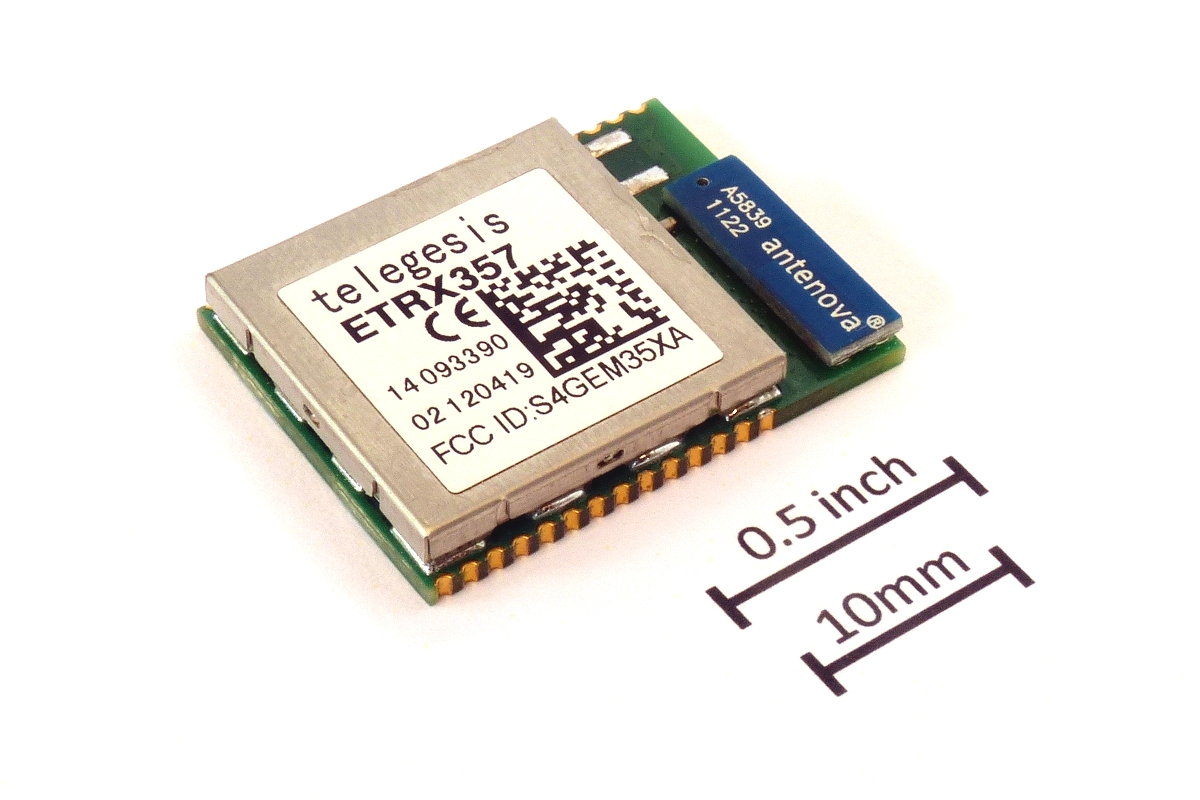
\includegraphics[height=2.5in]{figures/ETRX357_ZigBee_module_with_size_ref.jpg}
\caption[Modulo transductor de 2.4Gh Zigbee ETRX357]{Modulo transductor de Zigbee\footnotemark}
\end{figure}

\vspace{1cm}

Un ejemplo más de soluciones \gls{iot} es \verb|6LoWPan| ofrece un eficiente uso del protocolo IPv6 sobre el estándar IEEE 802.15.4 a través de redes locales inalámbricas ideadas para actuar como despliegues de red en malla~\cite{montenegro2007rfc}. Entre sus usos mas comunes se encuentra la industria \gls{iot}, la agricultura inteligente y las smart home. Este protocolo dispone además de una capa de seguridad adicional basada en autenticación y cifrado AES-128. Esto permite implementar mecanismos adicionales como \gls{tls} o firma digital en las comunicaciones. Su uso se planifica en transferencia de pequeñas tasas de datos, pero como resultado reduce el consumo de los nodos de la red. La siguiente figura~\ref{6Lowpandeploy} extraída del articulo 'The analysis of 6LoWPAN technology' refleja un ejemplo de despliegue de esta tecnología~\cite{ma2008analysis}.

\begin{figure}[hbt!]
\centering
\label{6Lowpandeploy}
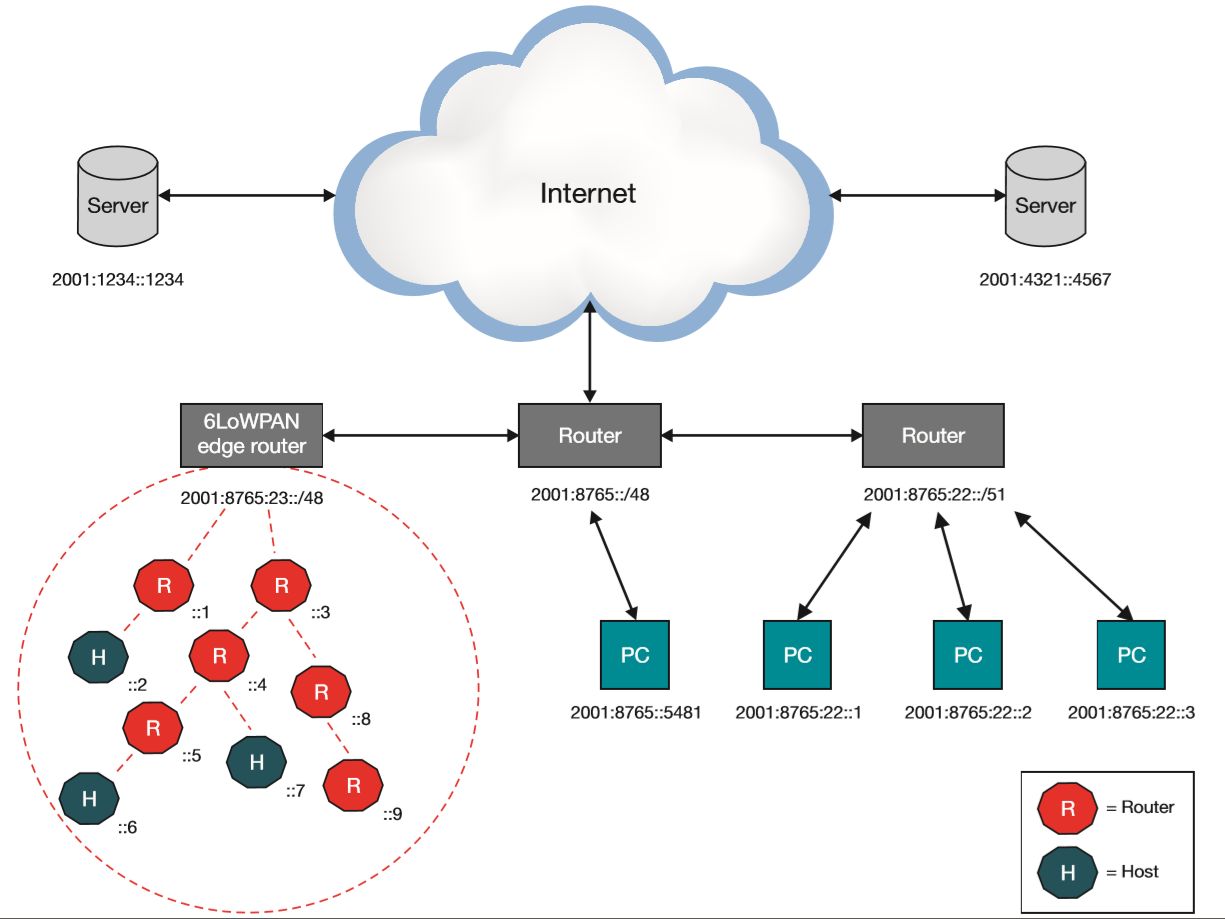
\includegraphics[height=5in]{figures/6LowPanDeploy.png}
\caption[Ejemplo de despliegue de una red 6LowPan con servicio en la nube]{Ejemplo de despliegue de una red 6LowPan con servicio en la nube}
\end{figure}

Otra de las tecnologías en {iot} es \verb|Lora|, su base tecnológica esta definida en el RFC8376~\cite{rfc8376} es el nombre común de la tecnología 'Low Power Wide Area Network' (LPWAN). Los despliegues de estas redes inalámbricas son de tipo estrella, pero la comunicación entre nodos y \gls{gateway} se establecen en canales individuales donde la velocidad de transferencia de datos se alcanza según la distancia entre dispositivos, la duración y consumo energético del mensaje a enviar. El efecto de esta técnica es que los canales con distintas velocidades de transferencia no interfieren entre si, lo cual genera un amplio abanico de canales simultáneos que pueden establecerse con el \gls{gateway}.

Otros protocolos interesantes son BLE, Wize o Sigfox.


\section{Hardware disponible}
\label{ch:Capitulo2.4}

Se han descrito algunas de las tecnologías características de las aplicaciones, topologías de red y protocolos de comunicación utilizados en domótica. Pero todo este entramado de software y señales deben operar en hardware físico. Más concretamente en múltiples dispositivos de hardware. En \gls{iot} el abanico de fabricantes de dispositivos orientados a sensorización y actuadores es tan extenso que simplemente está fuera de todo alcance el enumerarlos en este documento; aun así, considerando los objetivos definidos en el proyecto, que incluyen el uso de hardware open source, y costes de adquisición reducidos, podemos reducirlo a una lista de opciones acotada.

\vspace{1cm}

Es importante remarcar en este punto del documento, que en los proyectos de \gls{iot}, obtener el mejor balance de coste y eficiencia en la construcción es vital para soluciones profesionales. Para el prototipo que ocupa este proyecto, no se espera enfrentar este obstáculo, ya que no se encuentra definido en los objetivos el crear un sistema lo más equilibrado posible, sino uno funcional, respetando un límite de gasto que no supere la cuantía definida de 50 euros. Tampoco figura entre los objetivos asegurar un consumo energético los más reducido posible por parte de los dispositivos, pero se valorará la selección de equipamiento que, dando la mayor flexibilidad de configuración, se encuentre en valores de consumo lo suficientemente bajos como para que el prototipo sea fiable al ideal de una suite domótica funcional.

\vspace{1cm}

Partimos del concepto de suite domótica basado en dispositivos conectados a un nodo principal o \gls{gateway}, el cual actúa como router \gls{wifi}. Dicho \gls{gateway} posee un adaptador de red adicional que permite una conexión con la red de internet y que sea capaz de ejecutar servicios y aplicaciones actuando como servidor. Estos requisitos nos orientan a disponer de un ordenador completo, sera necesaria la flexibilidad de un SO que nos permita experimentar diferentes planteamientos, sin dejar de tener en cuenta que este ordenador tendrá una disponibilidad continua, y debe tener un consumo energético bajo y unos recursos suficientes para actuar como cimiento del prototipo.

\vspace{1cm}

Hace una década habría sido necesario apuntar a un equipo muy especializado y esto generalmente se traduce en un incremento del precio del equipo. Hoy, en cambio, disponemos de muchas opciones de ordenadores con un reducido factor de forma, bajo consumo eléctrico y recursos más que suficientes para cubrir muchos prototipos ligeros. Hablamos de la muy conocida Raspberry Pi y similares que has surgido con el tiempo (como Orange Pi, Banana Pi, Odroid o Matrix ARM ~\cite{lignuxComparative}), pueden encontrase en la figura \footnotetext{Comparativas de micro-ordenadores} algunos aspectos técnicos de sus capacidades comparadas entre sí.
. Para el caso que nos ocupa necesitamos que disponga de al menos dos adaptadores de red, uno de ellos inalámbrico, aunque puede subsanarse la falta del mismo mediante adaptadores inalámbricos USB (una estrategia muy común en los primeros modelos de Raspberry Pi hasta la serie 3). No es necesario que disponga de un procesador gráfico ya que operaremos de forma remota el ordenador mediante conexiones de SSH. Será un aspecto muy positivo que disponga de una interfaz para conectar dispositivos USB, este ultimo responde a la posible necesidad de conectar placas micro-controladoras para su programación.

\begin{figure}[hbt!]
\centering
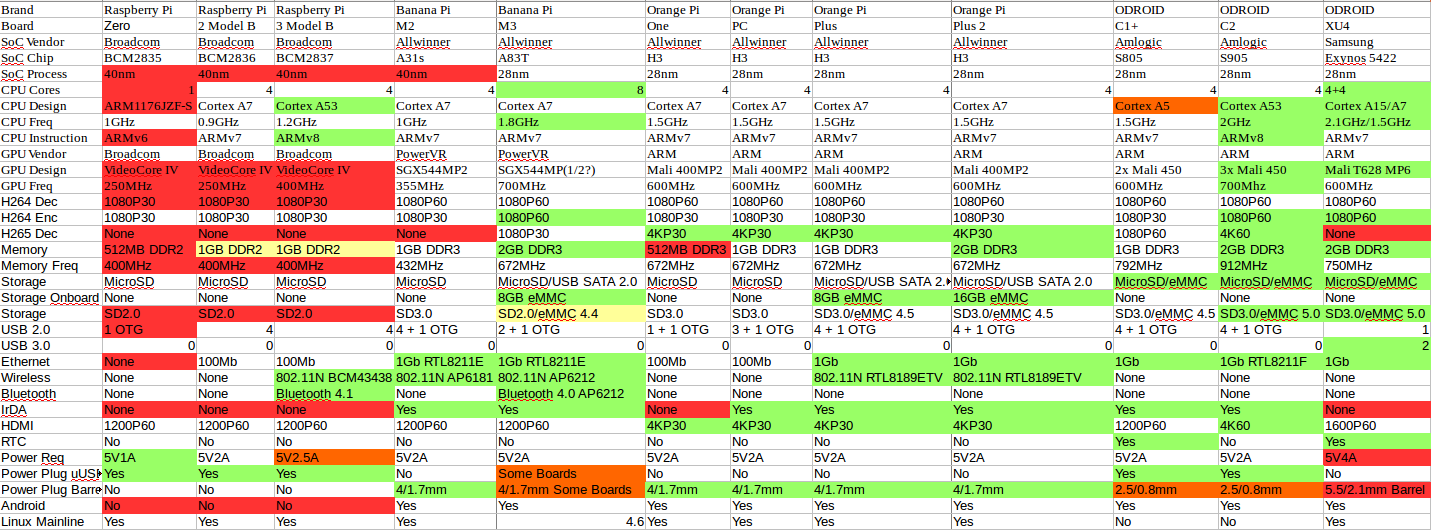
\includegraphics[height=2.5in]{figures/comparativaOrdenadores.png}
\caption[Comparativas de micro-ordenadores]{comparativa de características técnicas de micro-ordenadores\footnotemark}
\end{figure}


Raspberry Pi es posiblemente el uno de los mejores ejemplos de hardware abierto disponibles en el mercado. El diseño de su circuito impreso puede descargarse libremente para crear versiones modificadas.~\cite{raspberry_schematics}. Su precio puede variar notablemente dependiendo del vendedor, pero generalmente no debe superar los 35 euros. Dispone de capacidad suficiente para ejecutar distintos SO basados en arquitectura ARM. En el capítulo siguiente de la propuesta se evaluará que SO utilizar. De entre las distintas opciones disponibles, Raspberry Pi posee una de las comunidades de usuarios más grandes del mundo, posee una amigable documentación de uso e interminables ejemplos de uso y proyectos disponibles en la red. Sus especificaciones técnicas son suficientes para sostener los servicios necesarios para un prototipo de suite domótica, y puede alimentarse con una toma de USB de 5 Voltios.

\begin{figure}[hbt!]
\centering
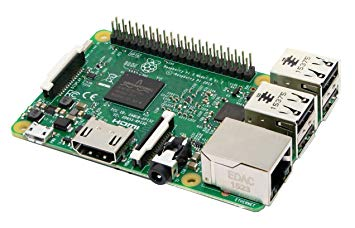
\includegraphics[height=2.5in]{figures/raspberrypi3b.jpg}
\caption[captura de una Raspberry]{Ordenador Raspberry Pi 3B\footnotemark}
\end{figure}

\vspace{1cm}


Esto cubriría el soporte físico necesario para crear un \gls{gateway}. Pero por sí solo no es suficiente. Los dispositivos que conectaremos a esta solución pueden presentarse en distintas opciones de hardware que pueden operar entre sí y con el propio \gls{gateway} mediante conectividad \gls{wifi}. Gracias a los protocolos de comunicación disponibles, un \gls{gateway} puede comunicarse con dispositivos de distintos fabricantes, presentando en la aplicación a todos ellos como dispositivos homogéneos con diferentes funciones.

\vspace{1cm}

En esencia, la clasificación de actores que conforman la red domótica se dividen en el \gls{gateway} (aunque pueden existir varios), los sensores y los actuadores. De hecho, un actuador no está restringido a actuar también como sensor y viceversa. Esta clasificación responde a la facilidad de entender rápidamente si un dispositivo actúa como entrada o salida del sistema. En \gls{iot} es habitual disponer de hardware especializado de bajo consumo y orientado a protocolo concretos de comunicación para ser usados en \gls{framework}, como ocurre con OpenHab, que facilita bastante la tarea de incluir nuevos dispositivos a la suite domótica si el producto a integrar ya está implementado. Si se desea disponer de la flexibilidad de cambiar radicalmente el comportamiento de un actor, modificando su comportamiento y hardware, es mejor plantear el uso de placas microcontroladoras programables.

\vspace{1cm}


Uno de los ejemplos mas conocidos y amigables de usar en placas micro-controladoras programables es Arduino. Estas placas disponen de conexiones \gls{io} que pueden usarse para ampliar su abanico e capacidades técnicas, en prototipos de \gls{iot}, es habitual dotar a una placa con conectividad \gls{wifi} mediante un adaptador inalámbrico conocido como shield.

\vspace{1cm}

En los últimos años ha aparecido un pequeño microcontrolador con chip de \gls{wifi} conocido generalmente como modulo ESP-01. Este chip permite una comunicación con el protocolo TCP/IP en una red inalámbrica. Se clasifica como hardware RF/IF y RFID CI de transceptor RF, capaz de operar con el protocolo 802.11b/g/n de 2.4GHz. El modelo ESP8266 que actualmente se comercializa posee capacidades superiores a su predecesora ESP8265 incluye una mayor capacidad de memoria flash interna, suficiente para abordar la mayoría de dispositivos \gls{iot} que pretendan actuar como actuadores o sensores.
Sin embargo, trabajar y programar estos chips puede resultar engorroso si no se dispone de USB con interfaz para escritura en serie, también puede hacerse con una placa de Arduino separando la cucaracha del microcontrolador del Arduino y cableando la conexión necesaria para programarse desde un ordenador.

\begin{figure}[hbt!]
\centering
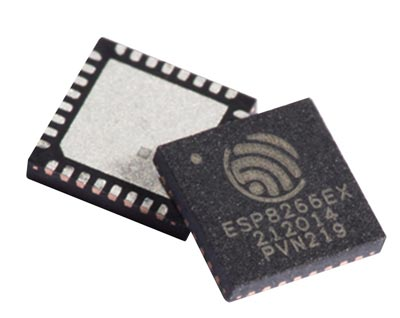
\includegraphics[height=2.5in]{figures/esp8266ex.jpg}
\caption[controladora ESP8233]{controladora ESP8266\footnotemark}
\end{figure}

\vspace{1cm}

Este microcontrolador opera con apenas 3.3VDC, lo cual es considerado como una ventaja a la hora de incluir este modulo en proyectos que operan sobre otras placas micro-controladoras como Arduino. Sin embargo, esta opción es válida sólo para la creación de prototipos funcionales, ya que el modulo ESP-01 requiere de un amperaje de al menos 200mAh para operar con normalidad. Los pines de alimentación de 3,3V de placas como Arduino ofrecen unos 50mAh de intensidad de corriente. Esto es suficiente para que el modulo opere, pero ocasionalmente puede causar daños en el modulo y generalmente el funcionamiento de la conexión es de baja calidad, con poca intensidad de señal, perdidas de paquetes y caídas de la conexión. La estrategia más extendida en facilitar una conexión estable de alimentación al modulo separado de la alimentación recibida por la placa microcontroladora en la que opera.

\vspace{1cm}

También pueden ejecutarse construcciones simples en una breadboard para un divisor de potencia mediante resistencias que transforme la señal de 5V de las placas microcontroladores, que habitualmente ofrecen un mayor valor de amperios, para dar una señal de 3.3VDC con mas de 200mA. Siendo realistas, no es ni siquiera necesario crearlos si se considera las opciones de venta de algunos fabricantes que montan una microcontrolador con chip ESP8266 en una ensamblada con las resistencias necesarias, interruptores y habitualmente sensores o actuadores como el mostrado en la imagen siguiente\footnotetext{ESP-01S con relé} a modo de módulo compacto alimentado por pines a 5V. El precio de estos módulos apenas alcanza un par de euros si se solicita a vendedores chinos, pero, es conveniente entender los riesgos que se asume al adquirir estos dispositivos de fabricantes clónicos con dudosos controles de calidad, que pueden seleccionar componentes incompatibles son redes \gls{wifi} como el suministrado por el adaptador inalámbrico de una Raspberry Pi 3B. Más información sobre estos problemas están ampliados en anexo B de troubleshooting.

\begin{figure}[hbt!]
\centering
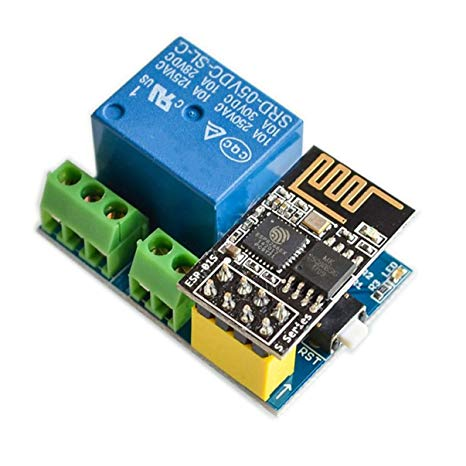
\includegraphics[height=2.5in]{figures/esp8266exRele.jpg}
\caption[ESP-01S con rele]{ESP8266 5V Modulo Rele\footnotemark}
\end{figure}

\vspace{1cm}

Con las complicaciones de alimentación del modulo \verb|ESP8266| surge al poco tiempo su sucesor natural, las placas nodeMCU. Conocidas por ser plataformas de código abierto para \gls{iot} más versátiles y accesibles en coste de adquisición. Uno de los aspectos que popularizó estos dispositivos fue la posterior portabilidad de la biblioteca de \gls{mqtt}, permitiendo al LUA de la \gls{soc} desplegar dicho protocolo. Aunque el proyecto de mantenimiento de firmware fue abandonado en 2015 por los autores originales, la comunidad de usuarios siguió mejorando el código hasta fecha de hoy, convirtiendo el nodeMCU en uno de los dispositivos mas demandados en proyectos, gracias a su bajo coste de precio, inferior a una decena de euros por placa, que dispone de 12 pines de \gls{gpio} permitiendo implementaciones complejas que aprovechan la conectividad inalámbricas para proyectos de \gls{iot}.

\begin{figure}[hbt!]
\centering
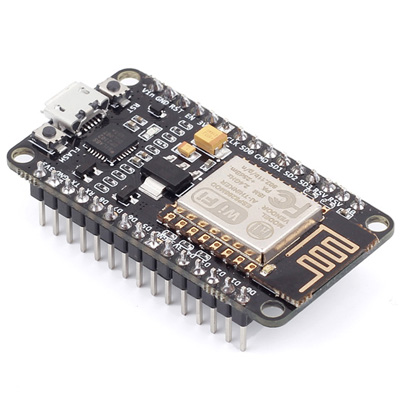
\includegraphics[height=2.5in]{figures/nodemcu.jpg}
\caption[captura de una nodeMCU]{Microcontroladora NodeMCU\footnotemark}
\end{figure}